\documentclass[tikz,border=10pt]{standalone}
\usetikzlibrary{calc,angles}
\begin{document}
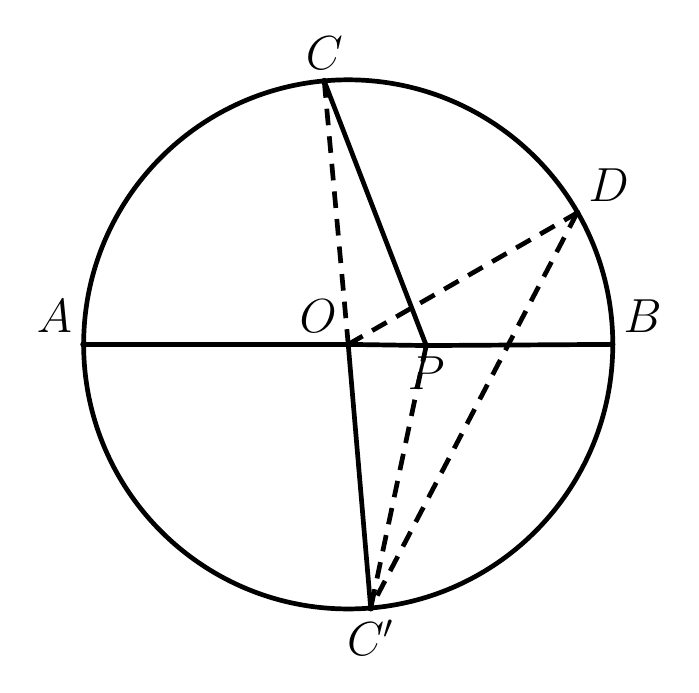
\begin{tikzpicture}[line width=1.7pt, line join=round]
\coordinate (A) at (-3.384,0.032);
\coordinate (B) at (3.328,0.032);
\coordinate (C) at (-0.327,3.375);
\coordinate (D) at (2.884,1.702);
\coordinate (O) at (-0.023,0.032);
\coordinate (P) at (0.968,0.017);




\coordinate (Cp) at (0.263,-3.318);


\draw (O) circle (3.360);


\draw[solid] (A) -- (O);
\draw[solid] (O) -- (P);
\draw[solid] (P) -- (B);
\draw[solid] (C) -- (P);
\draw[solid] (O) -- (Cp);


\draw[dash pattern=on 6pt off 4pt] (C) -- (O);
\draw[dash pattern=on 6pt off 4pt] (O) -- (D);
\draw[dash pattern=on 6pt off 4pt] (P) -- (Cp);
\draw[dash pattern=on 6pt off 4pt] (D) -- (Cp);


\foreach \q in {A,B,C,D,O,P,Cp} \fill (\q) circle (1.200pt);


\node[above left, font=\fontsize{18}{21.6}\selectfont] at (A) {$A$};
\node[above right, font=\fontsize{18}{21.6}\selectfont] at (B) {$B$};
\node[above, font=\fontsize{18}{21.6}\selectfont] at (C) {$C$};
\node[below, font=\fontsize{18}{21.6}\selectfont] at (Cp) {$C'$};
\node[above right, font=\fontsize{18}{21.6}\selectfont] at (D) {$D$};
\node[above left, font=\fontsize{18}{21.6}\selectfont] at (O) {$O$};
\node[below, font=\fontsize{18}{21.6}\selectfont] at (P) {$P$};
\end{tikzpicture}
\end{document}